% ============================================================================
% nbc_2026_core.tex
% CORE slide deck for the invited talk at the Nanyang Blockchain Conference
% 2026 (NTU Singapore, 21--22 August 2026). Built from the winning framing
% (output/nbc_pipeline/02_framings/framing_1.md) and the Phase-4/5 verified
% evidence under output/nbc_pipeline/04_evidence/. Do not add numbers to this
% file that are not traceable to those verified sources.
%
% Classical-Beamer skeleton per output/nbc_pipeline/00_exemplars.md: title ->
% abstract-bridge -> outline -> content under a persistent section header ->
% recap -> backup. One exhibit per slide; no dense equations live; tables are
% built directly from the verified .md evidence files (booktabs), not from
% the pre-redesign output/tables/*.pdf figures (those predate the 2026-08-04
% redesign and are explicitly not pre-cleared per framing_1.md Sec. 2).
%
% NOT YET COMPILED. Next phase: latexmk build + visual QA pass.
% ============================================================================
\documentclass[aspectratio=169]{beamer}

\usepackage[T1]{fontenc}
\usepackage{lmodern}
\usepackage{amsmath}
\usepackage{amssymb}
\usepackage{booktabs}
\usepackage{array}
\usepackage{multirow}
\usepackage{graphicx}
\usepackage{grffile}
\usepackage{tikz}
\usetikzlibrary{arrows.meta,positioning}

% ---------------------------------------------------------------------------
% Plain, light template. No heavy theme, no running logo (branding note:
% UCL CBT logo appears ONLY on the title slide via \titlegraphic below).
% ---------------------------------------------------------------------------
\usetheme{default}
\usecolortheme{default}
\setbeamertemplate{navigation symbols}{}
\setbeamertemplate{footline}{%
  \begin{beamercolorbox}[wd=\paperwidth,ht=2.6ex,dp=1.2ex,leftskip=.4cm,rightskip=.4cm]{structure}
    \usebeamerfont{footline}\scriptsize\insertsectionhead\hfill\insertframenumber\,/\,\inserttotalframenumber
  \end{beamercolorbox}%
}
\setbeamertemplate{itemize items}[circle]
\setbeamerfont{footline}{size=\scriptsize}

\tikzset{
  box/.style={draw, thick, rounded corners, align=center, font=\footnotesize,
              minimum width=3.3cm, minimum height=1.05cm, inner sep=3pt},
  arr/.style={-{Latex[length=2.2mm]}, thick}
}

\title[Vehicle Currencies in DeFi]{The Making of Vehicle Currencies}
\subtitle{Liquidity Provision in DeFi/AMM Markets}
\author[J.~Xu et al.]{Jiahua Xu \\ {\small with Emre Ozdenoren, Kathy Yuan, and Benjamin Chen}}
\institute{UCL Centre for Blockchain Technologies}
\date{Nanyang Blockchain Conference 2026 \\ NTU Singapore \\ 21--22 August 2026}

% ---------------------------------------------------------------------------
% Title-slide logo only (branding note: every other slide stays plain, no
% running footer logo). The path contains a literal, unescaped "&" (normally
% catcode 4, the alignment-tab character), which would misparse inside a
% macro argument. \newcommand/\titlegraphic tokenize their argument at the
% point the line is READ, so the catcode change must be a standalone
% top-level command executed immediately before that line, not nested
% inside the argument being defined -- then restored immediately after,
% since "&" is needed as a real alignment tab in every table later in this
% deck. Verified the logo file exists on disk (2026-08-04) before wiring
% this path.
% ---------------------------------------------------------------------------
\catcode`\&=12\relax
\titlegraphic{\includegraphics[width=3.4cm]{/Users/dsf-pro16-m3/Library/CloudStorage/OneDrive-SharedLibraries-UniversityCollegeLondon/UCL CBT - Documents/Operations (internal)/Media & Identity/Logos/Centre for Blockchain/Full colour/UCL_S_2C_DP_RGB_Ctr_Block_Tech_logos.png}}
\catcode`\&=4\relax

\begin{document}

% ============================================================================
% TITLE
% ============================================================================
\begin{frame}
  \titlepage
\end{frame}

% ============================================================================
% ABSTRACT-BRIDGING SLIDE
% Per framing_1.md Sec. 4 (as amended): Slide 2, immediately after the title
% and immediately before the outline. Content matches the four specified
% lines and footer; wording adjusted only to clear the cosmetic-language
% gate (no em-dashes, no "rather than", at most one "X, not Y" in the deck).
% ============================================================================
\begin{frame}{From the abstract to this talk}
  \begin{itemize}
    \item The NBC abstract described three roles: quoting/invoicing, vehicle/intermediation, and reserve/settlement, with a flight-to-dominance story under stress.
    \item[] \vspace{-0.3em}
    \item \textbf{This talk keeps only the vehicle/intermediation role, grounding it in liquidity provision instead of asset-pricing or flight dynamics.}
    \item[] \vspace{-0.3em}
    \item Dropped: the quoting/invoicing and reserve/settlement roles, and any claim about flight-to-dominance as a pricing or attack phenomenon.
    \item[] \vspace{-0.3em}
    \item What ``flight-to-dominance'' becomes here: liquidity depth and routing volume move together in the data (Proposition 1, with one contra-result left unresolved); architecture improves execution quality without changing which asset serves as the vehicle (Proposition 2).
  \end{itemize}
  \vfill
  {\scriptsize The full three-role framing remains the long-run agenda. Today's talk covers the liquidity-provision leg only.}
\end{frame}

% ============================================================================
% OUTLINE (manual list -- core sections only, backup excluded)
% ============================================================================
\begin{frame}{Outline}
  \begin{enumerate}
    \item Motivation
    \item The two propositions and their limits
    \item Mechanism (borrowed theory, three analogies)
    \item Evidence: formation (Proposition 1)
    \item Evidence: architecture (Proposition 2)
    \item Recap and contribution
  \end{enumerate}
\end{frame}

% ============================================================================
% 1. MOTIVATION
% ============================================================================
\section{Motivation}

\begin{frame}{Motivation: a vehicle-currency fact from FX}
  \begin{itemize}
    \item In interdealer FX, roughly \textbf{13\%} of USD-pair volume is vehicle-currency routing, a price-impact channel distinct from a spread-reducing one, rising to \textbf{25--38\%} in major pairs (Somogyi 2026, quasi-experimental holiday design).
    \item That paper's own panel-regression mechanism test (its C1--C3 specifications) is explicitly non-causal, with an $R^2$ of roughly 18--20\% dominated by fixed effects. We treat that mechanism test only as motivation; this talk does not rely on it as evidence.
  \end{itemize}
  \vspace{1em}
  \begin{block}{The pivot}
    In FX, vehicle status is usually read off fundamental dollar demand. In DeFi, transaction-level liquidity-provision data lets us ask directly whether it instead traces to liquidity provision itself.
  \end{block}
\end{frame}

% ============================================================================
% 2. THE TWO PROPOSITIONS AND THEIR LIMITS
% ============================================================================
\section{The two propositions}

\begin{frame}{The two propositions and their limits}
  \begin{block}{Proposition 1 (formation)}
    Vehicle-currency status is a liquidity-provision equilibrium: LP capital concentrates on a candidate's pools, deepens the pool, lowers the cost of indirect routing through it, and draws more LP capital, closing a self-reinforcing loop.
  \end{block}
  \begin{block}{Proposition 2 (architecture)}
    Architecture that cheapens LP repositioning makes vehicle status more elastic to stress.
  \end{block}
  \vspace{0.5em}
  \begin{alertblock}{Two constraints, named before the data}
    \small
    \textbf{P1:} no true exogenous shock is available in this sample. The one clean candidate (the UNI liquidity-mining launch, Sept.\ 2020) predates this repo's V3-only liquidity construction; what follows here is a lead-lag panel.\\
    \textbf{P2:} a 2021 market-wide volatility episode sits on the same date used to test P2 (the V2$\to$V3 launch), and this design cannot separate a true architecture effect from that episode in this sample.
  \end{alertblock}
\end{frame}

% ============================================================================
% 3. MECHANISM SCAFFOLD (three slides, one analogy each, borrowed theory)
% ============================================================================
\section{Mechanism (borrowed theory)}

\begin{frame}{Mechanism 1: the vehicle feedback loop (Krugman 1980, analogy)}
  \begin{center}
  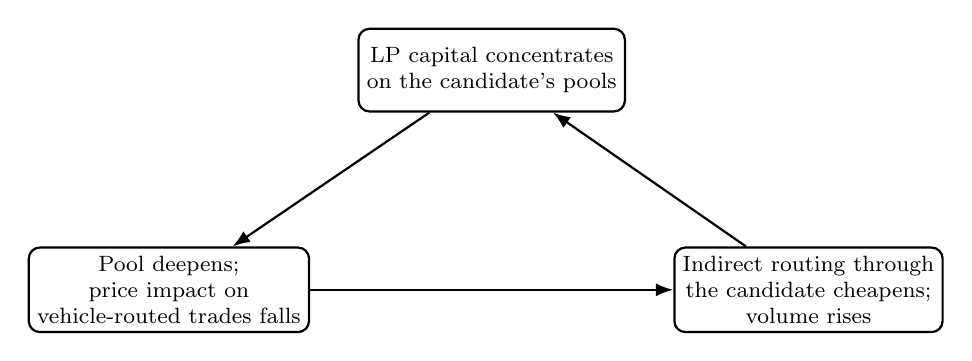
\begin{tikzpicture}[node distance=1.3cm and 1.0cm]
    \node[box] (A) {LP capital concentrates\\on the candidate's pools};
    \node[box, below left=1.7cm and 0.6cm of A] (B) {Pool deepens;\\price impact on\\vehicle-routed trades falls};
    \node[box, below right=1.7cm and 0.6cm of A] (C) {Indirect routing through\\the candidate cheapens;\\volume rises};
    \draw[arr] (A) -- (B);
    \draw[arr] (B) -- (C);
    \draw[arr] (C) -- (A);
  \end{tikzpicture}
  \end{center}
  {\footnotesize Motivating analogy only. Krugman's three-country transaction-cost mechanism, with an endogenized cost function. Scope here: at most three currencies, no persistence-after-dominance-fades claim, no empirical claim.}
\end{frame}

\begin{frame}{Mechanism 2: pool size and price impact (Leh\'ar \& Parlour 2024, analogy)}
  \begin{center}
  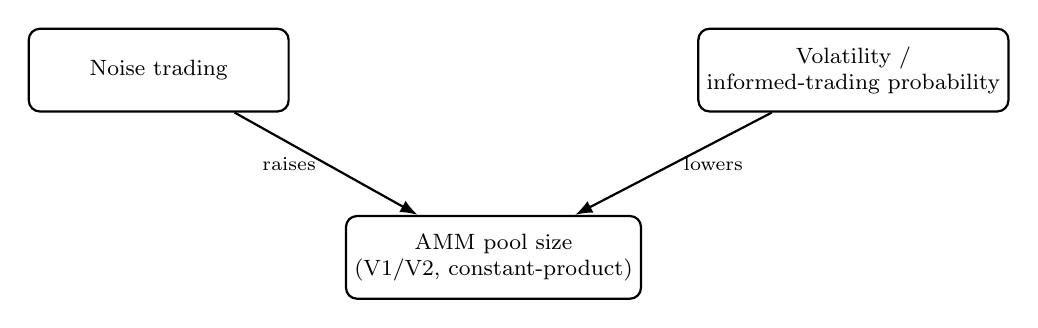
\begin{tikzpicture}[node distance=1.2cm and 1.0cm]
    \node[box] (P) {AMM pool size\\(V1/V2, constant-product)};
    \node[box, above left=1.3cm and 0.7cm of P] (N) {Noise trading};
    \node[box, above right=1.3cm and 0.7cm of P] (V) {Volatility /\\informed-trading probability};
    \draw[arr] (N) -- node[left, font=\scriptsize] {raises} (P);
    \draw[arr] (V) -- node[right, font=\scriptsize] {lowers} (P);
  \end{tikzpicture}
  \end{center}
  {\footnotesize Cited only for their own result: under bounded conditions, AMM price impact can be lower and less volatile than a comparable limit-order book. Scope: their own 43-pair Binance comparison, constant-product V1/V2 only. This talk does not extend that result to a general AMM-versus-order-book claim or to V3.}
\end{frame}

\begin{frame}{Mechanism 3: benchmark liquidity (Yuan 2005, analogy)}
  \begin{center}
  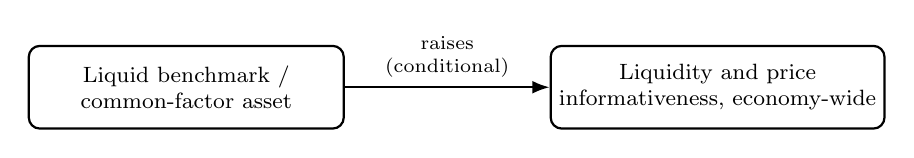
\begin{tikzpicture}[node distance=1.0cm and 1.6cm]
    \node[box, minimum width=4cm] (Y) {Liquid benchmark /\\common-factor asset};
    \node[box, minimum width=4cm, right=2.6cm of Y] (Z) {Liquidity and price\\informativeness, economy-wide};
    \draw[arr] (Y) -- node[above, font=\scriptsize, align=center] {raises\\(conditional)} (Z);
  \end{tikzpicture}
  \end{center}
  {\footnotesize Flagged as theory only, conditional on the specific assumption that market makers observe order flow across markets: no DeFi claim, no empirical claim, no assumption-free law.}
\end{frame}

% ============================================================================
% 4. EVIDENCE: FORMATION (P1)
% ============================================================================
\section{Evidence: formation (P1)}

\begin{frame}{Testing P1 with a lead-lag panel}
  \begin{itemize}
    \item \textbf{Sample:} 5 candidates (WETH, USDC, USDT, DAI, WBTC), daily, 2021-05-05 to 2026-06-30, balanced (1{,}883 dates $\times$ 5 tokens, $N=9{,}415$).
    \item \textbf{Three series per token-day:} $L$ = log candidate-linked liquidity; $D$ = DirectCostAdvantage (execution-cost gap, direct vs.\ indirect route); $S$ = indirect-route VehicleShare.
    \item \textbf{Design:} $\Delta_\tau(\text{outcome})_{t+\tau}$ on $L_t, D_t, S_t$, token $+$ date fixed effects, $\tau \in \{1,7,14,30\}$ days; cluster-by-date, Driscoll-Kraay, and month block-bootstrap inference.
    \item \textbf{What this shows:} $L$, $D$, $S$ at $t$ carry predictive content for each other's future changes beyond fixed effects. It cannot rule out a persistent common shock driving them together.
    \item \textbf{Independently re-derived} from scratch by two methods (sparse LSDV; from-scratch sandwich estimator); matches to 4 decimal places.
  \end{itemize}
\end{frame}

\begin{frame}{P1 headline: two legs support the loop, one is null, one runs backward}
  \small
  \begin{center}
  \begin{tabular}{@{}p{3.6cm}c p{5.1cm} l@{}}
    \toprule
    Relationship & Pred.\ sign & Evidence across the 4 horizons & Verdict \\
    \midrule
    $S$ on $L$ & $+$ & positive; $p<0.001$ (DK) at all 4 & \textbf{Robust} \\
    $L$ on $S$ & $+$ & positive; $p<0.05$ (DK) at 3 of 4 & Partial \\
    $S$ on $D$ & $-$ & correct sign; $p=0.06$--$0.24$, never sig. & Null \\
    $D$ on $L$ & $-$ & \textbf{wrong sign} at all 4; $p<0.06$ (DK) at 2 of 4 & \textbf{Contra} \\
    \bottomrule
  \end{tabular}
  \end{center}
  \vspace{0.6em}
  {\footnotesize ``$Y$ on $X$'' = outcome $Y_{t+\tau}$ regressed on $X_t$. Full table in backup. Two bars this design does not clear: no exogenous shock/IV, and the fourth prediction runs backward (next slide).}
\end{frame}

\begin{frame}{P1's contra-result: one leg of the loop runs backward}
  P1 predicts deeper own liquidity should \emph{lower} DirectCostAdvantage ($D$ on $L$, $\beta<0$). The pooled estimate is significantly positive at every horizon. This survives every robustness check we ran:
  \begin{itemize}
    \item Recurs in the low-baseline-depth subsample.
    \item Recurs in \emph{both} calm and high-volatility regimes.
    \item Recurs in 3 of 4 alternative depth/cost-measure constructions (the \$100k common-support variant is the one exception: it turns null instead of wrong-signed).
    \item Recurs in the pre-midpoint half of the sample.
  \end{itemize}
  \vspace{0.6em}
  \begin{alertblock}{Bottom line}
    Two of four legs of the proposed loop show lead-lag support ($S$ on $L$ robust, $L$ on $S$ partial); one is null; one runs opposite to the theory and stays unresolved.
  \end{alertblock}
\end{frame}

% ============================================================================
% 5. EVIDENCE: ARCHITECTURE (P2)
% ============================================================================
\section{Evidence: architecture (P2)}

\begin{frame}{Testing P2: V2 to V3 as an event study, reframed}
  \begin{itemize}
    \item \textbf{Original ask:} does architecture that cheapens LP repositioning make vehicle status more elastic to stress? Tested via the V2$\to$V3 concentrated-liquidity launch (2021-05-05).
    \item \textbf{Design note:} a cross-chain design was scoped and found not closeable (no multi-chain/L2 fetch path in this repo). Within-chain is the intended design, with chronological sample splits as the robustness check.
    \item \textbf{Sample:} 5 candidates, balanced pairs around the launch: $\pm$12 months (396 pairs, $N=65{,}022$) and $\pm$24 months (507 pairs, $N=97{,}484$).
    \item \textbf{Outcomes:} vehicle-candidate route share, vehicle HHI, direct-pool depth (level difference-in-differences), plus an elasticity test on $|$day-to-day change$|$ pre- vs.\ post-launch.
  \end{itemize}
\end{frame}

\begin{frame}{P2 headline: capital efficiency moves, topology does not}
  \small
  \begin{center}
  \begin{tabular}{@{}l l r r@{}}
    \toprule
    Window & Outcome & Effect & $p$ \\
    \midrule
    $\pm$12mo & Vehicle-candidate route share (pp) & 0.94 & 0.141 \\
    $\pm$12mo & Vehicle HHI & 0.014 & 0.246 \\
    $\pm$12mo & \textbf{Direct-pool depth (ratio)} & \textbf{0.120} & \textbf{$<$0.001} \\
    \midrule
    $\pm$24mo & Vehicle-candidate route share (pp) & 1.13 & 0.123 \\
    $\pm$24mo & Vehicle HHI & 0.023 & 0.131 \\
    $\pm$24mo & \textbf{Direct-pool depth (ratio)} & \textbf{0.120} & \textbf{$<$0.001} \\
    \bottomrule
  \end{tabular}
  \end{center}
  \vspace{0.6em}
  Direct-pool depth improves significantly post-V3 in both windows. Route share and vehicle HHI do not move. Architecture that improves execution quality does not automatically change which asset serves as the vehicle.
\end{frame}

\begin{frame}{Why the elasticity claim is not testable here}
  \begin{columns}[T]
    \begin{column}{0.52\textwidth}
      \small
      Monthly mean $|$day-to-day $\Delta$ route share$|$, model-free, from the raw panel:
      \begin{center}
      \begin{tabular}{@{}l r@{}}
        \toprule
        Month & pp \\
        \midrule
        2020-12 & 16.5 \\
        2021-01 & 21.4 \\
        2021-05 (launch) & 22.2 (peak) \\
        2021-06 & 16.8 \\
        \bottomrule
      \end{tabular}
      \end{center}
      {\footnotesize Matches the well-documented Jan--May 2021 alt-season volatility episode, unrelated to the AMM architecture change.}
    \end{column}
    \begin{column}{0.48\textwidth}
      \small
      \begin{itemize}
        \item Pre-launch placebo dates: large, significant ``elasticity'' jumps ($t=4.4$--$7.8$).
        \item Post-launch placebos: mostly null.
        \item True launch window sits at the peak of the same cycle and comes back null.
        \item Joint pretrend Wald test: $\chi^2=49$--$67$, $p<0.001$ for every outcome, while the linear pretrend slope is insignificant ($p=0.14$--$0.99$), consistent with a step-like calendar effect.
      \end{itemize}
      \vspace{0.4em}
      Not identifiable in this sample by this design. Not claimed either way.
    \end{column}
  \end{columns}
\end{frame}

% ============================================================================
% 6. RECAP
% ============================================================================
\section{Recap}

\begin{frame}{Recap and contribution}
  \begin{itemize}
    \item Liquidity depth and routing volume move together in the direction P1 predicts ($S$ on $L$ robust across every check), with one contra-result left unresolved ($D$ on $L$, wrong-signed and robust to being wrong).
    \item Architecture that improves execution quality (direct-pool depth up 0.12, $p<0.001$) does not change which asset serves as the vehicle (route share and HHI both null); the P2 elasticity claim cannot be identified in this sample given a diagnosed 2021 confound.
    \item Capital efficiency and vehicle-currency status are separable margins.
  \end{itemize}
  \vspace{0.8em}
  \begin{block}{}
    \centering A modest, partially-supported finding, not a closed causal loop.
  \end{block}
\end{frame}

% ============================================================================
% BACKUP
% ============================================================================
\section{Backup}

\begin{frame}
  \centering
  \vfill
  {\Large \textbf{Backup}}
  \vspace{1em}

  {\small
  Full P1 headline table \quad $\vert$ \quad P1 robustness detail \\
  P2 sample and level DiD \quad $\vert$ \quad P2 placebo/pretrend \\
  P2 volatility split and version construction \quad $\vert$ \quad References
  }
  \vfill
\end{frame}

\begin{frame}{Backup: P1 full headline panel (all four relationships)}
  \tiny
  \begin{center}
  \begin{tabular}{@{}l c r r r l@{}}
    \toprule
    Relationship & $\tau$ (days) & $\beta$ & SE (DK) & $p$ (DK) & Sign check \\
    \midrule
    $S$ on $L$ & 1  & 0.0223  & 0.0015 & $<$0.001 & match \\
    $S$ on $L$ & 7  & 0.0261  & 0.0023 & $<$0.001 & match \\
    $S$ on $L$ & 14 & 0.0270  & 0.0030 & $<$0.001 & match \\
    $S$ on $L$ & 30 & 0.0270  & 0.0036 & $<$0.001 & match \\
    \midrule
    $L$ on $S$ & 1  & 0.0189  & 0.0095 & 0.046 & match \\
    $L$ on $S$ & 7  & 0.0377  & 0.0146 & 0.010 & match \\
    $L$ on $S$ & 14 & 0.0483  & 0.0247 & 0.051 & marginal \\
    $L$ on $S$ & 30 & 0.0842  & 0.0344 & 0.014 & match \\
    \midrule
    $S$ on $D$ & 1  & $-$0.0060 & 0.0036 & 0.095 & sign only \\
    $S$ on $D$ & 7  & $-$0.0057 & 0.0049 & 0.239 & sign only \\
    $S$ on $D$ & 14 & $-$0.0122 & 0.0065 & 0.060 & sign only \\
    $S$ on $D$ & 30 & $-$0.0129 & 0.0084 & 0.123 & sign only \\
    \midrule
    $D$ on $L$ & 1  & 0.0111  & 0.0054 & 0.039 & \textbf{wrong sign} \\
    $D$ on $L$ & 7  & 0.0162  & 0.0085 & 0.057 & \textbf{wrong sign} \\
    $D$ on $L$ & 14 & 0.0168  & 0.0113 & 0.139 & \textbf{wrong sign} \\
    $D$ on $L$ & 30 & 0.0244  & 0.0154 & 0.113 & \textbf{wrong sign} \\
    \bottomrule
  \end{tabular}
  \end{center}
  \vspace{0.4em}
  \tiny Predicted signs: $S$ on $L$ ($+$), $L$ on $S$ ($+$), $S$ on $D$ ($-$), $D$ on $L$ ($-$). $N=9{,}265$--$9{,}410$; 1{,}853--1{,}882 date clusters. Source: \texttt{04\_evidence/p1/p1\_headline\_panel\_results.md}, independently re-derived (Sec.\ 5).
\end{frame}

\begin{frame}{Backup: P1 robustness battery detail}
  \footnotesize
  \begin{itemize}
    \item \textbf{Subsample sign-check tallies} across depth / volatility / alt-measure / period splits (144 alt-measure cells; 72 each for depth, volatility, period): $D$ on $L$ wrong-signed in 6, 8, 13, and 5 cells respectively. It never disappears; it only occasionally turns null.
    \item \textbf{Volatility split example} ($D$ on $L$, $\tau=1$): calm $\beta=0.0071$ ($p=0.409$); high $\beta=0.0117$ ($p=0.106$): same wrong sign in both regimes.
    \item \textbf{Alt-measure example} ($D$ on $L$, winsorized-mean $D$, $\tau=1$): $\beta=0.0133$, $p<0.001$: wrong sign, now significant.
    \item \textbf{LINK falsification/placebo} (non-candidate token, own-series, $N=8$ cells): sign matches the pooled headline in only 4/8 cells; LINK's own coefficients are indistinguishable from zero in 7/8 ($p>0.15$); one cell has the wrong sign at $p=0.036$. Too noisy for a clean placebo pass either way.
    \item \textbf{Period split:} $S$ on $L$ holds in both halves ($\beta=0.022$--$0.026$ pre, $0.052$--$0.062$ post); $D$ on $L$'s wrong sign appears pre-midpoint too ($p=0.09$--$0.18$).
  \end{itemize}
  {\scriptsize Source: \texttt{04\_evidence/p1/p1\_robustness\_battery\_summary.md}.}
\end{frame}

\begin{frame}{Backup: P2 sample and level DiD (both windows)}
  \footnotesize
  \begin{center}
  \begin{tabular}{@{}l r r r r@{}}
    \toprule
    Window & Balanced pairs & Pair-day rows & First date & Last date \\
    \midrule
    $\pm$12mo & 396 & 32{,}557 & 2020-05-19 & 2022-05-05 \\
    $\pm$24mo & 507 & 48{,}319 & 2020-05-19 & 2023-05-05 \\
    \bottomrule
  \end{tabular}
  \end{center}
  \vspace{0.6em}
  \begin{center}
  \begin{tabular}{@{}l l r r r r@{}}
    \toprule
    Window & Outcome & Effect & SE & $t$ & $p$ \\
    \midrule
    $\pm$12mo & Route share (pp) & 0.9448 & 0.6402 & 1.48 & 0.141 \\
    $\pm$12mo & Vehicle HHI & 0.0143 & 0.0123 & 1.16 & 0.246 \\
    $\pm$12mo & Direct-pool depth & 0.1203 & 0.0257 & 4.68 & $<$0.001 \\
    $\pm$24mo & Route share (pp) & 1.1276 & 0.7298 & 1.55 & 0.123 \\
    $\pm$24mo & Vehicle HHI & 0.0226 & 0.0150 & 1.51 & 0.131 \\
    $\pm$24mo & Direct-pool depth & 0.1201 & 0.0275 & 4.36 & $<$0.001 \\
    \bottomrule
  \end{tabular}
  \end{center}
  {\scriptsize Elasticity test ($|$day-to-day change$|$, pre vs.\ post) on the same outcomes: all 6 cells null, $p=0.25$--$0.94$. Source: \texttt{04\_evidence/p2/p2\_vehicle\_status\_elasticity\_results.md}.}
\end{frame}

\begin{frame}{Backup: P2 placebo dates and joint pretrend tests}
  \footnotesize
  \begin{center}
  \begin{tabular}{@{}l l r r@{}}
    \toprule
    Placebo date & Regime & Elasticity effect (route share, pp) & $p$ \\
    \midrule
    2020-10-01 & pre-launch placebo & 3.4318 & $<$0.001 \\
    2020-11-15 & pre-launch placebo & 4.0151 & $<$0.001 \\
    2021-01-01 & pre-launch placebo & 5.9643 & $<$0.001 \\
    2021-05-05 & \textbf{true launch} ($\pm$12mo) & $-$0.6810 & 0.621 \\
    2022-05-05 & post-launch placebo (+1y) & $-$0.6550 & 0.427 \\
    2023-05-05 & post-launch placebo (+2y) & 1.1534 & 0.135 \\
    \bottomrule
  \end{tabular}
  \end{center}
  \vspace{0.5em}
  \textbf{Joint pretrend Wald test} (pre-launch month dummies jointly zero), route share: $\pm$12mo $\chi^2=64.24$, $p<0.001$ (linear slope $p=0.994$); $\pm$24mo $\chi^2=67.48$, $p<0.001$ (linear slope $p=0.836$). This joint rejection alongside a flat linear slope is a step-like calendar effect, the same signature a market-wide volatility episode would produce.\\
  {\scriptsize Source: \texttt{04\_evidence/p2/p2\_robustness\_battery\_results.md}. Sec.\ 5's independent code audit plus raw-panel recomputation traces this to the design; no coding bug was found.}
\end{frame}

\begin{frame}{Backup: P2 volatility split and version construction}
  \footnotesize
  \begin{itemize}
    \item \textbf{Volatility split} (elasticity test, route share, $\pm$12mo): high pre-V3 volatility $\beta=0.40$ ($p=0.823$); low pre-V3 volatility $\beta=-1.15$ ($p=0.522$): null in both subsamples.
    \item \textbf{Version construction} (level DiD, direct-route availability, $\pm$12mo): best-across-versions $+11.1$pp ($p<0.001$); V2-only $-39.7$pp ($p<0.001$); V3-only $+50.8$pp ($p<0.001$): a mechanical availability shift, consistent with the reframed capital-efficiency reading and distinct from an independent elasticity result.
    \item Fixed 12- and 24-month windows reproduce the headline level-DiD and elasticity numbers exactly (robustness item iv).
  \end{itemize}
  {\scriptsize Source: \texttt{04\_evidence/p2/p2\_robustness\_battery\_results.md}.}
\end{frame}

\begin{frame}{References}
  \footnotesize
  \begin{itemize}
    \item Somogyi, F.\ (2026). FX vehicle-currency routing, quasi-experimental holiday design. Motivation only.
    \item Krugman, P.\ (1980). Three-country transaction-cost vehicle-selection mechanism. Motivating analogy for P1.
    \item Yuan, K.\ (2005). Benchmark/common-factor liquidity, conditional theory. Motivating analogy for P1.
    \item Leh\'ar, A.\ and Parlour, C.\ (2024). AMM (V1/V2) pool size and price impact vs.\ a limit order book. Motivating analogy for P1.
    \item Klein, O., Kozhan, R., Viswanath-Natraj, G., and Wang, J.\ (2026). LP minting/burning and short-horizon return predictability. Motivates strategic LP behavior behind P1.
    \item Caparros, B., Chaudhary, S., and Klein, O.\ (2024). Gas costs, LP repositioning, and liquidity concentration. Identification template for P2.
    \item Klein, O.\ and Song, Y.\ (2021); He, Z., Khorrami, P., and Song, Y.\ (2022). TradFi liquidity-commonality and intermediary-capacity analogies. Background only, no DeFi extension claimed.
  \end{itemize}
\end{frame}

\end{document}
